\graphicspath{{figures/results/}}
\chapter{Results}
The results presented are both training and testing results from the two solutions. Both the image classification bound occlusion detection and the multi-class object detection bound occlusion detection are trained and tested on the 60 seconds video with three fish.

It is trained on annotated data of around 200 different occlusions in total and annotated "no occlusions".
%The results presented are made by labelling all occlusions happening in the data. This covers the two videos provided by Loligo Systems which include three and five fish, each just about one minute long. The labelling is done by marking the point in which an occlusion is spotted, with skeletons drawn on each image. The frames of the video in which no occlusions occur does not have any labelling.
%
\section{Image Classification}
The image classification is trained for 15 epochs.
\begin{figure}[H]
	\centering
	\begin{subfigure}{0.48\textwidth}
		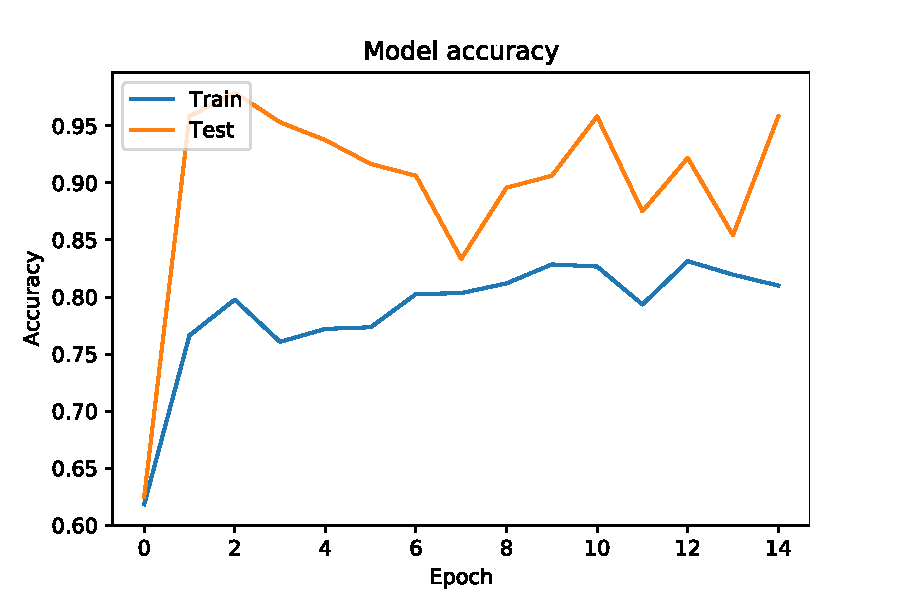
\includegraphics[width=\textwidth]{model_acc_15epoch}
		\caption{The image classification accuracy for both training and testing}
		\label{fig:img_acc}
	\end{subfigure}
	\begin{subfigure}{0.48\textwidth}
		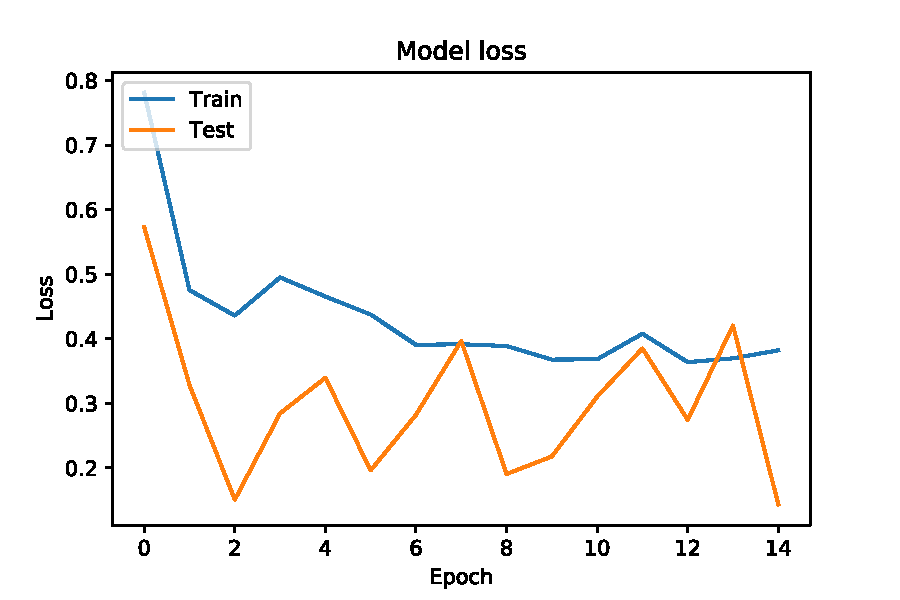
\includegraphics[width=\textwidth]{model_loss_15epoch}
		\caption{The image classification loss for both training and testing}
		\label{fig:img_loss}
	\end{subfigure}
\end{figure}
The model here achieves: 
\begin{table}[]
	\centering
	\caption{Results achieved with 15 epochs.}
	\begin{tabular}{|l|l|}
		\hline
		Loss                & 0.4841 \\\rowcolor{lightGrey}\hline
		Accuracy            & 0.7738 \\ \hline
		Validation Loss     & 0.2487 \\\rowcolor{lightGrey}\hline
		Validation Accuracy & 0.9318\\ \hline
	\end{tabular}
\label{tab:img_class_15ep}
\end{table}




\section{Object Detection}
\section{Training}



\subsection{40 Epochs}
\begin{figure}[H]
	\centering
	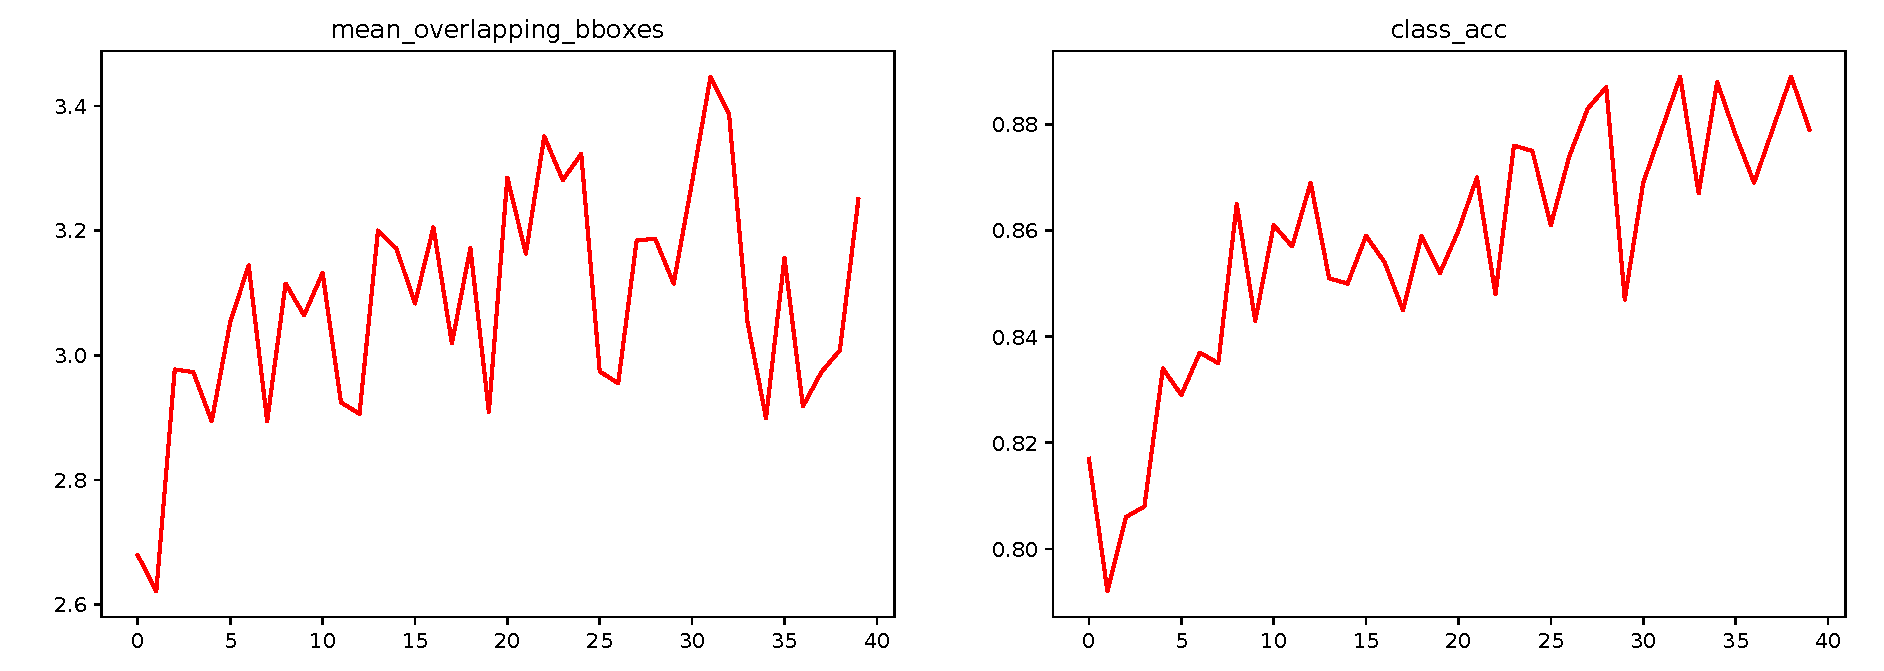
\includegraphics[width=\textwidth]{acc}
	\caption{Accuracy}
	\label{fig:}
\end{figure}
\begin{figure}[H]
	\centering
	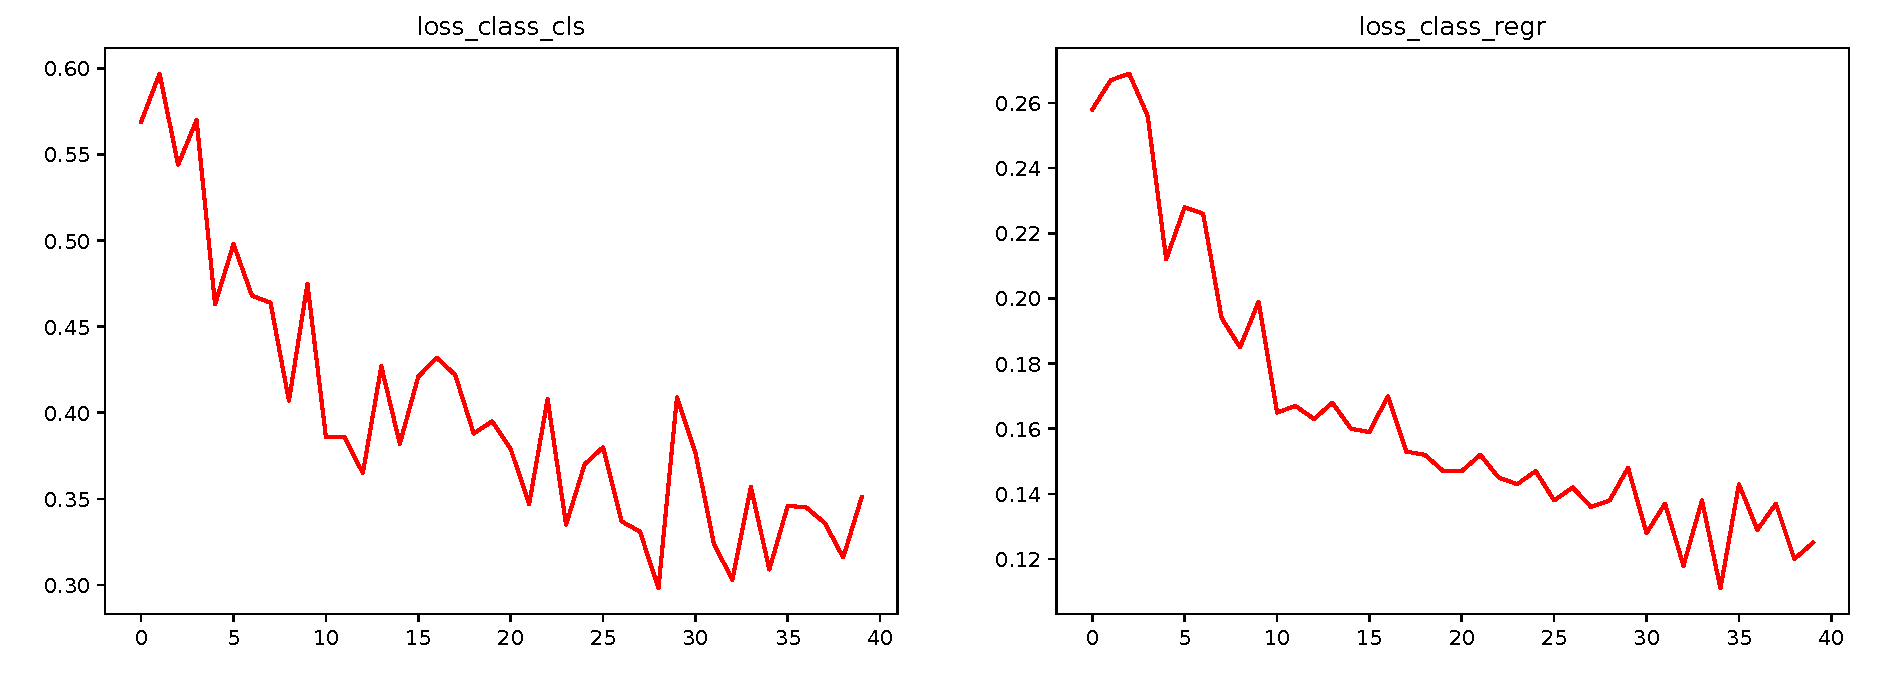
\includegraphics[width=\textwidth]{loss_class}
	\caption{Loss Class - classification and bbox regression}
	\label{fig:}
\end{figure}
\begin{figure}[H]
	\centering
	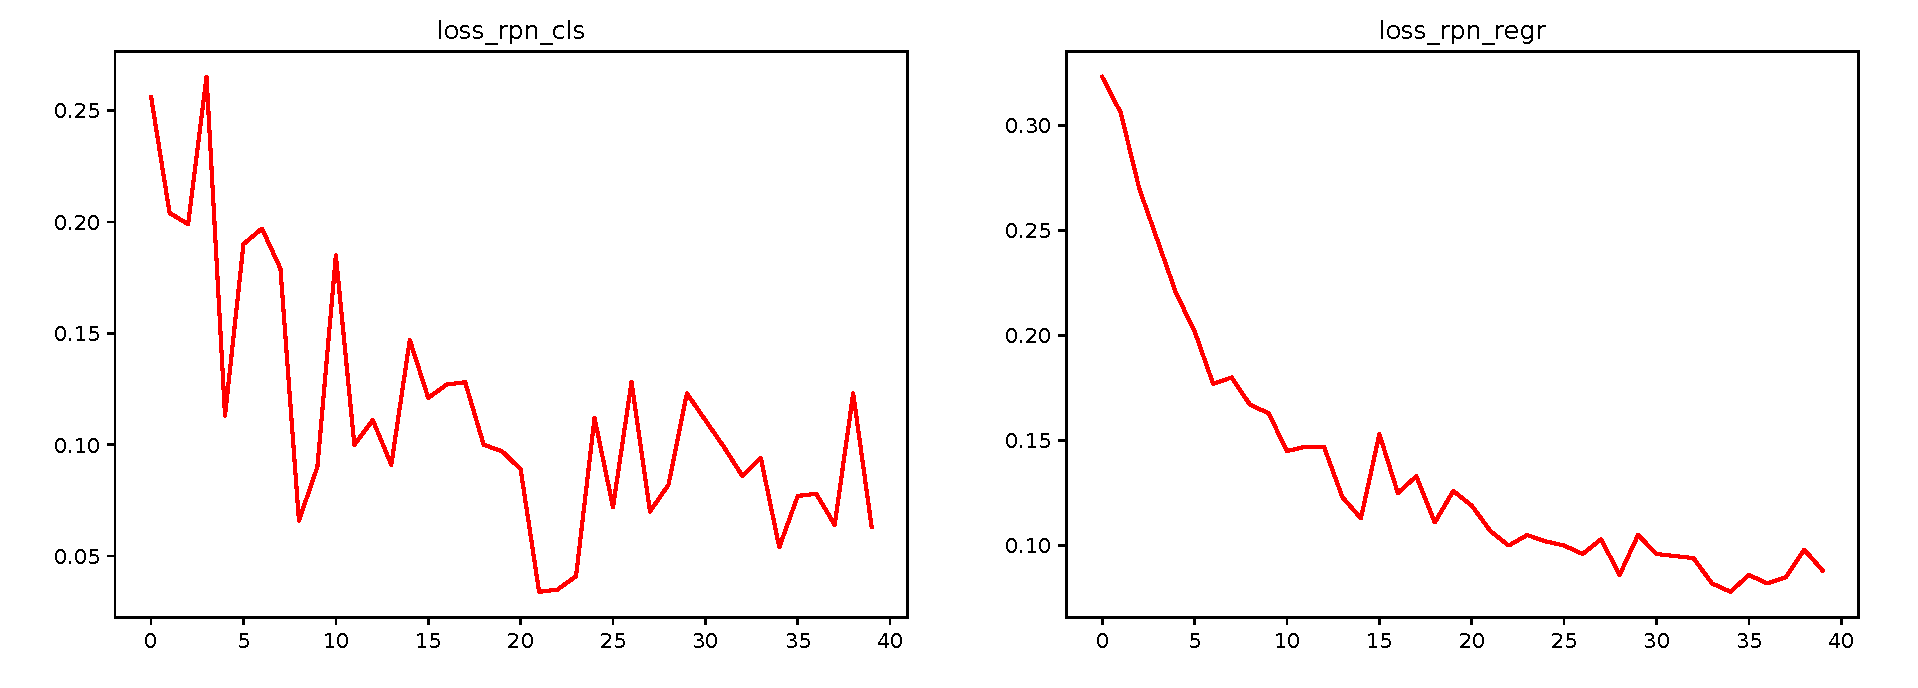
\includegraphics[width=\textwidth]{loss_rpn}
	\caption{Loss Region Proposal Network - classification and bbox regression}
	\label{fig:}
\end{figure}
\begin{figure}[H]
	\centering
	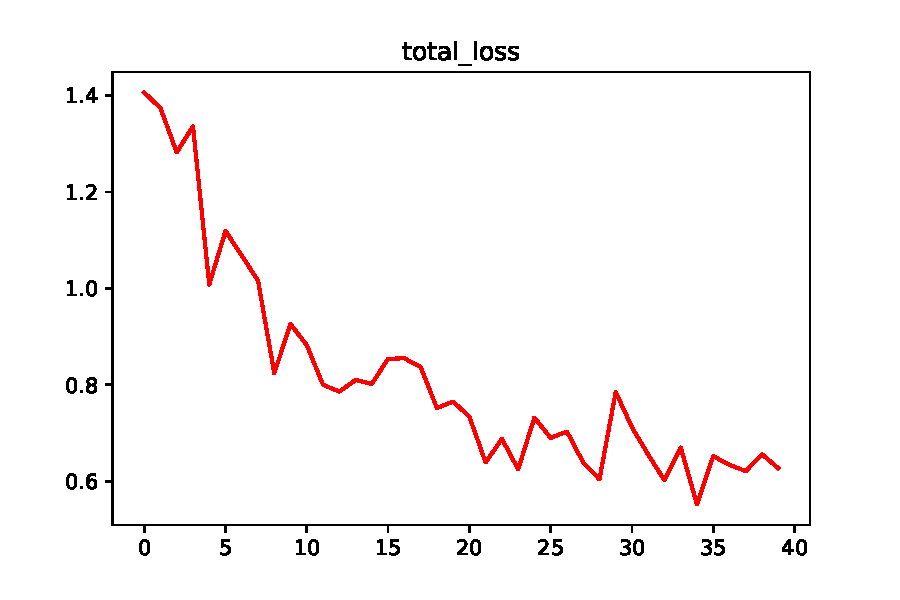
\includegraphics[width=0.85\textwidth]{total_loss}
	\caption{Total loss}
	\label{fig:}
\end{figure}

\subsection{135 Epochs}
\begin{figure}[H]
	\centering
	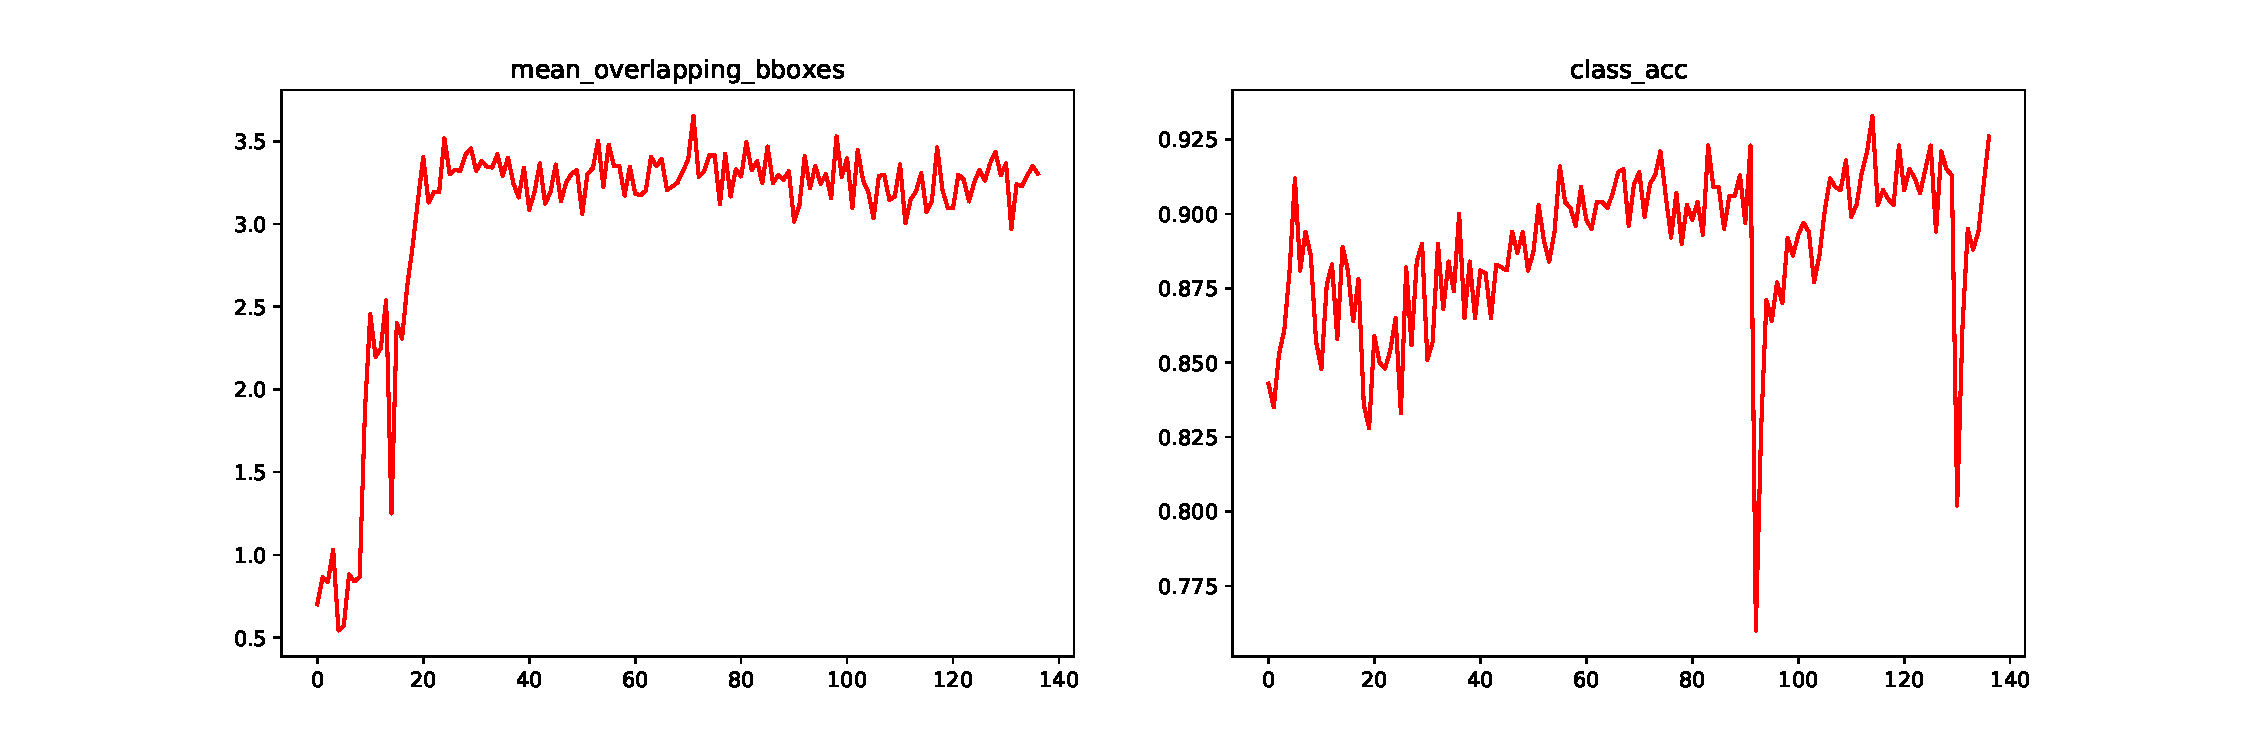
\includegraphics[width=\textwidth]{acc-135}
	\caption{Accuracy}
	\label{fig:}
\end{figure}
\begin{figure}[H]
	\centering
	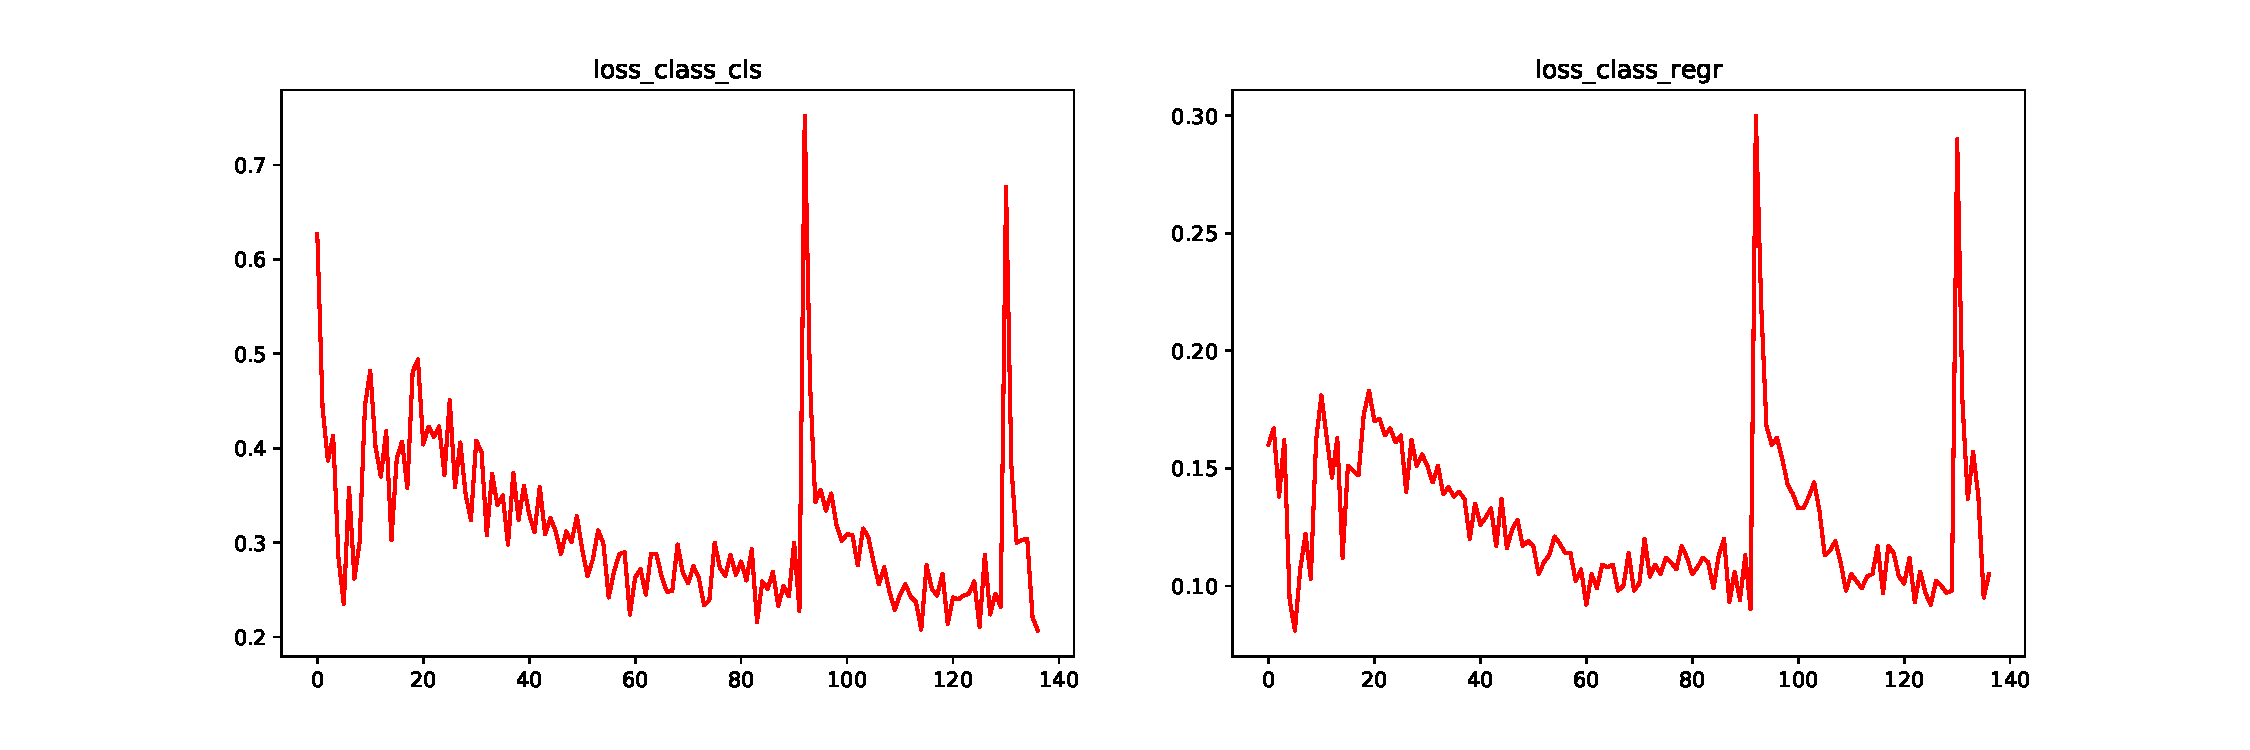
\includegraphics[width=\textwidth]{loss_class-135}
	\caption{Loss Class - classification and bbox regression}
	\label{fig:}
\end{figure}
\begin{figure}[H]
	\centering
	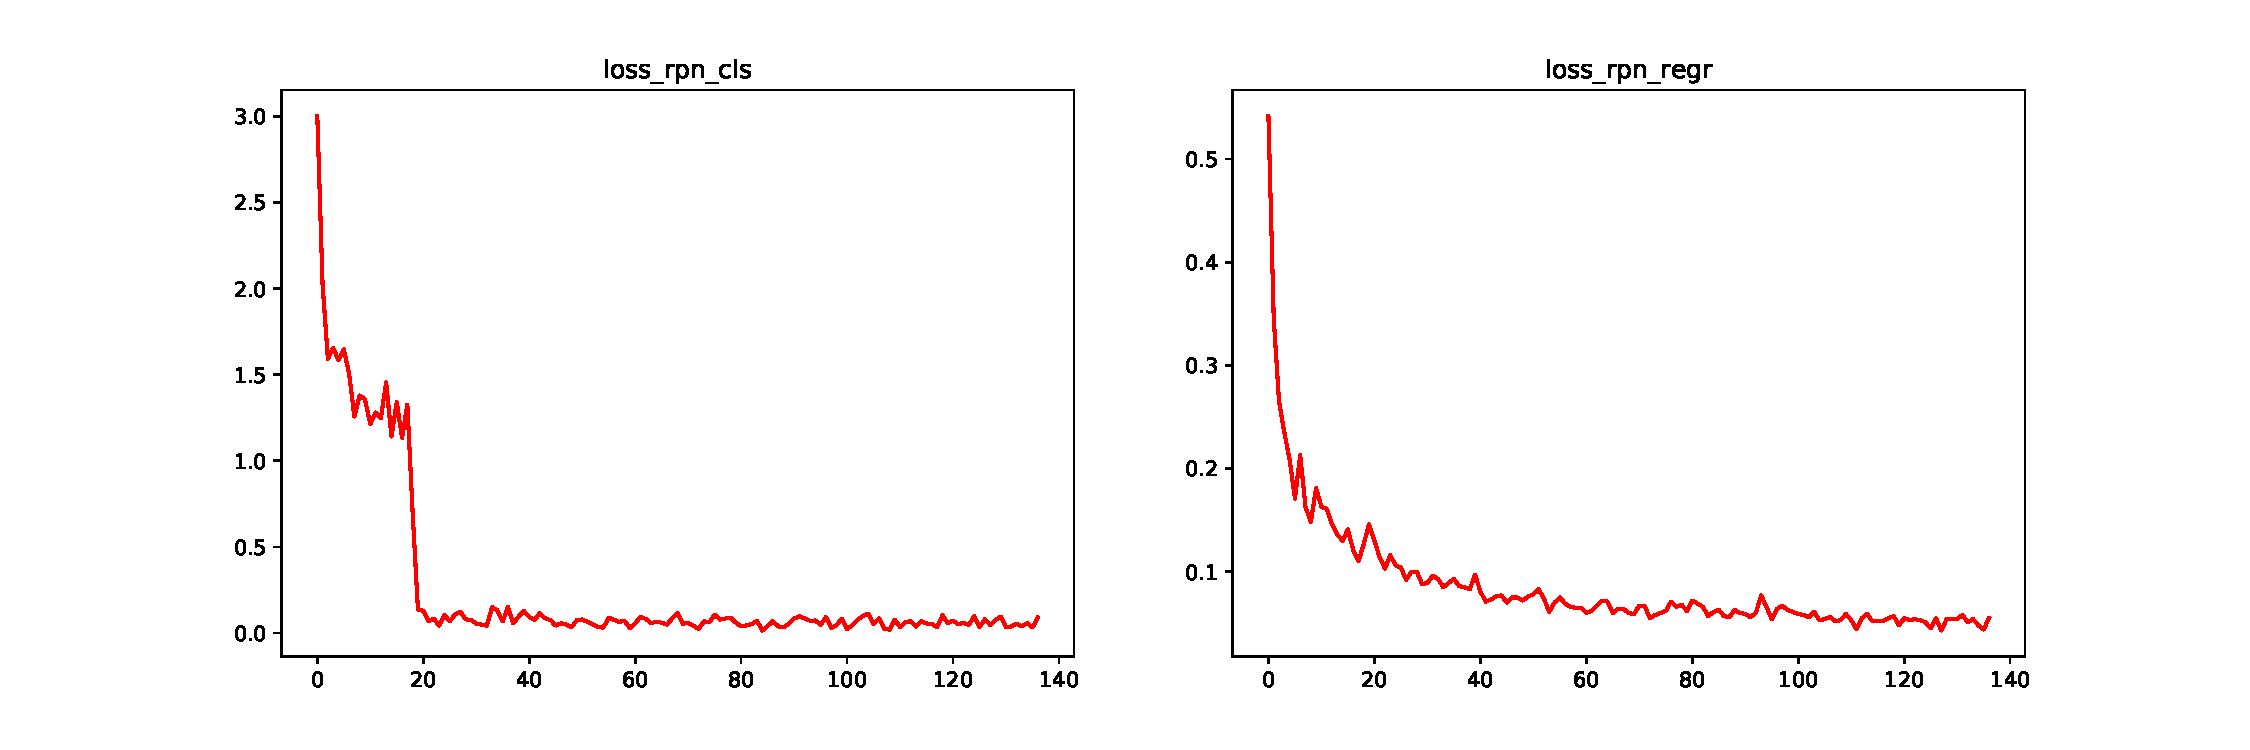
\includegraphics[width=\textwidth]{loss_rpn-135}
	\caption{Loss Region Proposal Network - classification and bbox regression}
	\label{fig:}
\end{figure}
\begin{figure}[H]
	\centering
	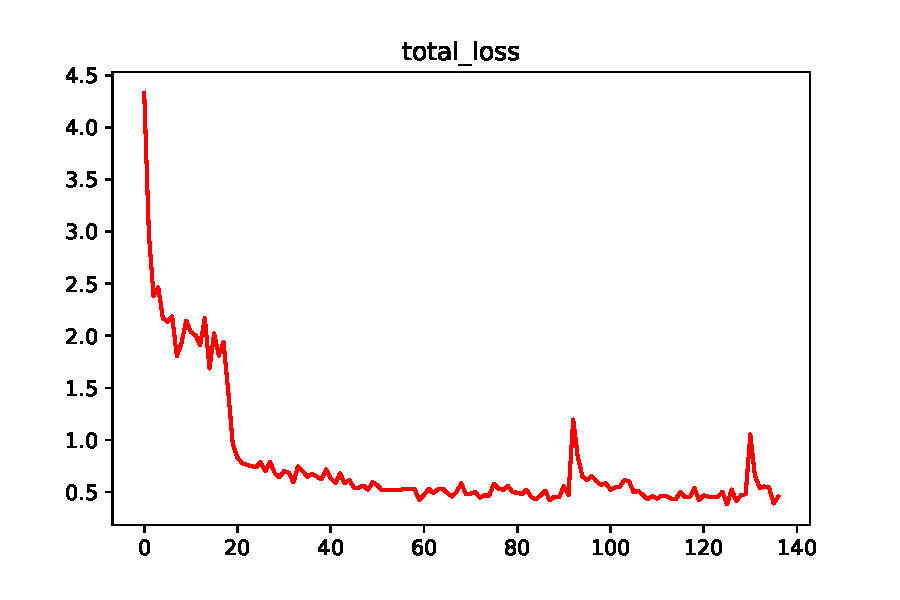
\includegraphics[width=0.7\textwidth]{total_loss-135}
	\caption{Total loss}
	\label{fig:}
\end{figure}


\section{Testing}
\gls{map} at $81.7\%$. \todo{Make figures showing detections}

%
%\section{Five Fish}